% ============================================================================
% Non-Exhaustive Common-Source Inertial Bridges in TCGS-SEQUENTION
% Conditional companion to the framework-independent quantized-inertia audit
% Copyright (c) 2026 Henry Arellano-Pena - CC BY 4.0
% ============================================================================

\documentclass[11pt]{article}

\usepackage[margin=1in]{geometry}
\usepackage[T1]{fontenc}
\usepackage[utf8]{inputenc}
\usepackage{lmodern}
\usepackage{microtype}
\usepackage{setspace}
\setstretch{1.055}

\usepackage{amsmath,amssymb,amsthm,mathtools,bm,mathrsfs}
\usepackage{siunitx}
\sisetup{detect-all,per-mode=symbol}

\usepackage{graphicx}
\usepackage{booktabs}
\usepackage{array}
\usepackage{tabularx}
\usepackage{longtable}
\usepackage{float}
\usepackage{caption}
\usepackage{enumitem}
\usepackage[most]{tcolorbox}
\usepackage{tikz}
\usetikzlibrary{arrows.meta,positioning,fit,calc}
\graphicspath{{figures/}}

\usepackage[numbers,sort&compress]{natbib}
\usepackage[hidelinks]{hyperref}
\usepackage[nameinlink,noabbrev]{cleveref}
\urlstyle{same}
\hypersetup{
  pdftitle={Non-Exhaustive Common-Source Inertial Bridges in TCGS-SEQUENTION: Identifiable Low-Rank Images, Anchored Coordinates, and Lossy Cross-Channel Tests},
  pdfauthor={Henry Arellano-Pena},
  pdfsubject={Conditional, identifiable, compressed, gauge-fixed, lossy cross-channel inertial bridges within TCGS-SEQUENTION},
  pdfkeywords={TCGS-SEQUENTION, Counterspace, Extrinsic Constitutive Law, inertia, common-source factorization, identifiable quotient, low rank, coordinate gauge, Moore-Penrose pseudoinverse, selector naturality, synthetic discrimination}
}

\newtheorem{definition}{Definition}
\newtheorem{principle}{Principle}
\newtheorem{criterion}{Criterion}
\newtheorem{assumption}{Assumption}
\newtheorem{protocol}{Protocol}
\newtheorem{remark}{Remark}
\newtheorem{lemma}{Lemma}

\newcommand{\Cfour}{\mathcal{C}_{4}}
\newcommand{\Shadow}{\Sigma_{3}}
\newcommand{\Sset}{\mathcal{S}}
\newcommand{\ECL}{\mathsf{E}}
\newcommand{\Info}{\operatorname{Info}}
\newcommand{\Read}{\operatorname{Read}_{\Sset,G}}
\newcommand{\Adm}{\operatorname{Adm}}
\newcommand{\ev}{\operatorname{ev}}
\newcommand{\phys}{\operatorname{phys}}
\newcommand{\dd}{\mathrm{d}}
\newcommand{\abs}[1]{\left\lvert #1\right\rvert}
\newcommand{\norm}[1]{\left\lVert #1\right\rVert}
\newcommand{\avg}[1]{\left\langle #1\right\rangle}
\newcommand{\Bdy}{\mathcal{B}}
\newcommand{\Corridor}{\mathfrak{c}}
\newcommand{\Carrier}{\kappa}
\newcommand{\Selector}{\sigma}
\newcommand{\QI}{\mathrm{QI}}
\newcommand{\ellR}{\ell_{\mathrm R}}
\newcommand{\LH}{L_{\mathrm H}}
\newcommand{\Mcal}{\mathcal{M}}
\newcommand{\Kout}{\mathcal{K}_{\mathrm{out}}}

\begin{document}

\title{\textbf{Non-Exhaustive Common-Source Inertial Bridges in TCGS--SEQUENTION:}\\
Identifiable Low-Rank Images, Anchored Coordinates, and Lossy Cross-Channel Tests}

\author{Henry Arellano-Pe\~na\\
Nuevo Estandar Biotropical NEBIOT S.A.S., Bogot\'a, Colombia\\
\texttt{harellano@unal.edu.co}}

\date{22 August 2026}
\maketitle

\begin{center}
\small
\textcopyright\ 2026 Henry Arellano-Pe\~na. This work is licensed under the Creative Commons Attribution 4.0 International License (CC BY 4.0).\\
\url{https://creativecommons.org/licenses/by/4.0/}
\end{center}

\begin{abstract}
A source--Shadow framework cannot acquire empirical content merely by factoring every carrier response through an unrestricted latent operator: any finite family of unrelated kernels admits an automatic block-diagonal realization. This paper develops a conditional and falsifiable inertial-sector bridge within TCGS--SEQUENTION while preserving the framework's non-exhaustive map discipline. The governing source ontology, the Extrinsic Constitutive Law (ECL), a finite bridge-coordinate representation, and any physical readout are assigned distinct jurisdictions. The finite latent spaces are therefore called \emph{shared bridge-coordinate spaces}, not the source itself. Their inner products, coordinate convention, admissible residual global gauge, and channel maps must be anchored either by a source-derived reduction or by an independent multi-channel calibration campaign completed before target anomalies are inspected. Per-channel coordinate gauges are forbidden.

For a preregistered channel portfolio, fixed channel maps define a linear observation operator on the rank-bounded bridge variety. The relevant complexity is not the nominal dimension of that variety but the dimension of its image in the channel portfolio, equivalently the dimension of the identifiable quotient after directions unseen by every channel are removed. A declared compression ratio and a separate parameter-to-calibration-data ceiling prevent nearly saturated constructions from masquerading as common-source compression. Held-out adequacy is tested through predictive covariance, Mahalanobis residuals, multiplicity control, and a preregistered power calculation against the null of independent per-channel kernels. Because no finite readout is assumed source-exhaustive, exact inverses are rejected. Moore--Penrose pseudoinverses reconstruct only partial operators on bridge sectors made readable by independently calibrated channel maps, and cross-channel consistency is evaluated only on a nontrivial shared reconstructible sector, where agreement is proved as a lemma requiring metric-orthogonal projectors rather than asserted. The observed channel kernels are Fr\'echet derivatives at declared base points, so the protocol tests linearized responses under a declared linearity tolerance and does not claim to test full nonlinear common-source structure.

A fully reproducible synthetic three-channel example demonstrates the forbidden region. Data generated from one rank-two bridge are accepted at the declared five-percent size, whereas independent channel kernels are rejected with unit empirical power in the reported Monte Carlo design. A near-saturated construction retaining 98 percent of unrestricted parameter capacity is rejected by the predeclared compression ceiling even though it satisfies a merely strict dimension inequality. Quantized inertia supplies a motivating case but no evidence for the framework: its laboratory proper-acceleration branch and galactic relational-acceleration branch remain different empirical laws until a covariant bridge is derived. Failure of the anchored low-rank image criterion, selector naturality, shared-sector consistency, or held-out predictive test rejects the inertial bridge proposed here. Success supports that bridge only; it does not automatically establish Counterspace, ECL, or non-ontic time.
\end{abstract}

\noindent\textbf{Keywords:} TCGS--SEQUENTION; Counterspace; Extrinsic Constitutive Law; inertia; common-source factorization; identifiable quotient; low-rank image; coordinate gauge; multi-channel calibration; Moore--Penrose pseudoinverse; selector naturality; synthetic discrimination; falsification.

\section*{Jurisdiction and relation to the independent QI audit}

This manuscript is the conditional TCGS companion to a framework-independent audit of quantized inertia (QI) \cite{ArellanoQIAudit2026}. The independent audit establishes its quantum-field-theoretic, covariance, algebraic, laboratory, and astrophysical conclusions without using TCGS--SEQUENTION. The present paper does not repeat those arguments and does not use their correctness as evidence for Counterspace. Conversely, TCGS is not used to repair a failed QI derivation.

The governing methodological separation is
\begin{equation}
\boxed{
\text{source architecture}
\neq
\text{inertial-sector bridge}
\neq
\text{QI reduction}
\neq
\text{one empirical readout}.
}
\label{eq:jurisdiction}
\end{equation}
The foundational framework already requires each response function, kernel, and numerical pipeline to remain open to derivational and empirical failure \cite{ArellanoFoundation2026}. The non-exhaustive map programme further denies that one finite readout can be identified with complete Territory \cite{ArellanoNoFinalMap2026}. The task here is therefore narrow: construct a finite, genuinely restrictive, lossy, and testable bridge that could connect one source-grounded inertial response to several physical channels without treating any channel as an exhaustive window on the source.

\section{Introduction}

A common-source explanation can fail in two opposite ways. It can be too rigid, demanding that every carrier reproduce one response exactly despite distinct preparation, constitutive, and measurement physics. Or it can be too permissive, declaring that all observed kernels ``factor through one source'' while allowing the source space and channel maps to be enlarged until the statement becomes an identity.

The second failure is especially subtle. Suppose a finite channel family has arbitrary kernels
\begin{equation}
K_{\chi}:\mathcal A_{\chi}\longrightarrow\mathcal F_{\chi}.
\end{equation}
If one defines
\begin{equation}
\mathcal H^{\mathrm{in}}_{\oplus}
:=\bigoplus_{\chi}\mathcal A_{\chi},
\qquad
\mathcal H^{\mathrm{out}}_{\oplus}
:=\bigoplus_{\chi}\mathcal F_{\chi},
\qquad
\mathbb K_{\oplus}:=\bigoplus_{\chi}K_{\chi},
\label{eq:trivial_direct_sum}
\end{equation}
then the canonical inclusion and projection maps satisfy
\begin{equation}
K_{\chi}
=P^{\mathrm{out}}_{\chi}\,
 \mathbb K_{\oplus}\,
 P^{\mathrm{in}}_{\chi}
\end{equation}
for every channel, whatever the kernels are. This construction defines no forbidden region and yields no evidence of a common physical source. It only repackages unrelated maps in one larger block-diagonal operator.

A scientifically meaningful source bridge must therefore impose restrictions that are fixed before target comparison and cannot be recreated by direct sum. It must also respect the framework's own epistemic limit: if finite Shadow maps are partial and generally many-to-one, no channel should be assumed to possess a two-sided inverse that reconstructs the complete source response.

This paper develops that correction. Its contributions are:
\begin{enumerate}[leftmargin=1.55em]
\item a typed placement of a finite inertial bridge downstream of the ECL without identifying the bridge coordinates with Counterspace;
\item an explicit analytic representation package for every derivative, norm, pseudoinverse, and operator claim;
\item an identifiable-image dimension that removes bridge directions invisible to the entire channel portfolio;
\item a preregistered compression ratio, data-capacity ceiling, and power requirement against independent channel kernels;
\item one globally shared bridge-coordinate convention, with only a common residual gauge and no per-channel gauge freedom;
\item two admissible anchoring routes: source-derived reduction or independent multi-channel calibration;
\item covariance-based held-out residual tests and lossy Moore--Penrose reconstruction on nontrivial shared readable sectors;
\item a reproducible synthetic acceptance--rejection demonstration;
\item selector naturality for equivalent presentations and an explicit separation of the laboratory and galactic branches of QI.
\end{enumerate}

\section{Governing TCGS--SEQUENTION architecture}

\subsection{Source, Shadow, and operational order}

TCGS--SEQUENTION distinguishes a complete non-temporal four-dimensional Counterspace \(\Cfour\) from an operationally real three-dimensional Shadow \(\Shadow\) \cite{ArellanoFoundation2026,ArellanoMinkowski2026}. Let
\begin{equation}
\mathfrak F
=\{X_{\lambda}:\Shadow\hookrightarrow\Cfour\}_{\lambda\in I}
\end{equation}
be an admissible family of embeddings or readout relations. The label \(\lambda\) is gauge under admissible monotone reparameterization; operational clocks and acceleration records are physical Shadow constructions. The source is not treated as a substance evolving through an ontic temporal coordinate.

This ontology does not abolish force, acceleration, momentum transfer, or measured inertia. Those remain physically real relations in the Shadow. It only prevents a finite carrier law from being identified directly with the complete source or with the ECL.

\subsection{Typed source-to-registration chain}

Let \(\Xi\in\mathfrak X_{\mathrm{adm}}\) be a complete admissible source configuration. The typed chain is
\begin{align}
M_{\Xi}&:=\Info(\Xi),\\
\ECL_{\Sset,\Xi}&:=\Read(M_{\Xi}),\\
\ECL^{\Selector}_{\Sset,\Xi}&:=\ev_{\Selector}(\ECL_{\Sset,\Xi}),\\
O_{\Selector,\Carrier,\Corridor}(\Xi)
&:=\pi^{\phys}_{\Selector,\Carrier,\Corridor}
  \left(\ECL^{\Selector}_{\Sset,\Xi}\right).
\label{eq:typed_chain}
\end{align}
Here \(M_{\Xi}\) is the non-experiential informational organization of the source, \(\ECL_{\Sset,\Xi}\) is the complete readability profile, \(\Selector\) selects one admissible presentation, \(\Carrier\) is the physical carrier, \(\Corridor\) specifies preparation and measurement, and \(O\) is the registered observable \cite{ArellanoECL2026,ArellanoInfoECL2026}. These objects are not interchangeable:
\begin{equation}
\Xi\neq M_{\Xi}\neq \ECL_{\Sset,\Xi}
\neq O_{\Selector,\Carrier,\Corridor}(\Xi).
\end{equation}

A finite inertial kernel belongs downstream of \(O\). It is a local analytic representation of how selected variations register in one physical corridor. It is not the ECL itself and does not add source content.

\subsection{Mass, inertia, and weight}

The independent TCGS treatment distinguishes mass as a projection-stable representation or spectral label, inertia as effective dynamical resistance in a declared corridor, and weight as the support reaction preventing free response in a gravitational environment \cite{ArellanoMassInertia2026}. Therefore
\begin{equation}
\text{mass}\neq\text{inertia}\neq\text{weight}\neq\text{ECL}.
\label{eq:mass_inertia_weight}
\end{equation}
A boundary-conditioned force anomaly does not by itself imply a change in ontological mass. It can arise from field momentum, material response, support compliance, carrier dynamics, or a genuine modification of inertial readout. The bridge must discriminate among those possibilities.

\section{QI as a motivating but non-governing case}

QI proposes
\begin{equation}
m_{\mathrm I}=m\left(1-\frac{2c^{2}}{|a|\Theta}\right),
\qquad
\eta_{\QI}:=\frac{m_{\mathrm I}}{m}
=1-\frac{a_{0}^{\QI}}{|a|},
\qquad
a_{0}^{\QI}:=\frac{2c^{2}}{\Theta}.
\label{eq:qi_scalar}
\end{equation}
Equivalently, with
\begin{equation}
\ellR:=\frac{c^{2}}{|a|},
\qquad
\LH:=\frac{\Theta}{2},
\end{equation}
one has
\begin{equation}
\eta_{\QI}=1-\frac{\ellR}{\LH}.
\label{eq:qi_ratio}
\end{equation}
Within TCGS this ratio may be read conditionally as an attenuation of effective projection stiffness,
\begin{equation}
\Mcal^{I}_{\mathrm{eff}}=m\eta_{\QI},
\end{equation}
but that reading is not a derivation from A1--A4. It does not establish that QI is an expression of ECL.

The word ``attenuation'' also requires care, and the independent audit supplies the reason \cite{ArellanoQIAudit2026}. \Cref{eq:qi_scalar} is implicit in \(a\): the effective mass depends on the acceleration and the acceleration depends on the effective mass. Read explicitly, with \(|a|\) supplied from outside, \(\eta_{\QI}\) is negative for \(|a|<a_{0}^{\QI}\) and is not an attenuation at all. Read implicitly, with \(|a|\) the realized acceleration, closing \(F=m_{\mathrm I}a\) gives
\begin{equation}
a=\frac{F}{m}+a_{0}^{\QI},
\qquad
\eta_{\QI}=\frac{F}{F+m\,a_{0}^{\QI}}\in[0,1),
\label{eq:qi_realized_companion}
\end{equation}
so the attenuation reading is correct, positivity is automatic, and the minimum acceleration is derived rather than posited. Only under the second reading is \(m\eta_{\QI}\) a legitimate stiffness. The distinction matters for the bridge because \cref{eq:qi_realized_companion} is a different function of the channel input than \cref{eq:qi_scalar} evaluated at a prescribed \(|a|\); a portfolio that linearizes one channel under one reading and another channel under the other is comparing derivatives of different maps and would violate \cref{sec:linearization}.

The independent audit identifies a decisive acceleration fork \cite{ArellanoQIAudit2026}. The ordinary Unruh relation uses proper four-acceleration
\begin{equation}
a^{\mu}_{\mathrm{prop}}=u^{\nu}\nabla_{\nu}u^{\mu},
\end{equation}
whereas QI's galactic applications use acceleration relative to surrounding matter \cite{McCulloch2016}. Field-emitted electrons in a capacitor can possess very large proper acceleration; a star following a galactic geodesic has vanishing proper acceleration even when its spatial coordinates exhibit orbital curvature. Until a covariant relational acceleration and its detector or horizon response are derived, the two empirical branches are
\begin{equation}
\QI_{\mathrm{lab}}[a_{\mathrm{prop}},\Bdy]
\quad\text{and}\quad
\QI_{\mathrm{gal}}[a_{\mathrm{rel}},\Theta],
\qquad
\QI_{\mathrm{lab}}\not\equiv\QI_{\mathrm{gal}}.
\label{eq:branch_split}
\end{equation}
A laboratory confirmation would not support the galactic law, and a galactic fit would not support the capacitor mechanism, unless both arise from one covariant action or response functional.

\section{Generic modified inertia and the location of TCGS content}

A history-dependent inertial law can be represented schematically by
\begin{equation}
F_i(\lambda)
=\int_{\Lambda}
K^{I}_{ij}(\lambda,\lambda';\mathcal D)
 a^{j}(\lambda')\,\dd\lambda'
+R_i(\lambda),
\label{eq:generic_kernel}
\end{equation}
where \(\mathcal D\) denotes declared carrier, boundary, state, and environmental data. This generic nonlocal form is not original to TCGS. Milgrom showed that modified-inertia actions with the relevant symmetry and conservation requirements are generically history-dependent and nonlocal \cite{Milgrom1994}. Positivity, regularity, causality, and memory are likewise ordinary effective-theory requirements.

The specifically TCGS content can therefore not be the mere existence of a kernel. It must be an additional restriction on the family of channel kernels generated from one source rule. The proposal developed below is one such conditional restriction: a finite set of carrier-specific kernels must lie in the identifiable low-dimensional image of one anchored, rank-bounded shared bridge and independently calibrated channel maps. The finite bridge is a representation of a jointly readable source-conditioned sector; it is not Counterspace or the complete ECL.

\section{Analytic representation package}

The four axioms do not by themselves provide Banach manifolds, tangent spaces, Hilbert norms, Fr\'echet derivatives, pseudoinverses, or finite empirical discretizations. Any use of a chain rule or operator factorization requires these structures to be declared explicitly.

\begin{assumption}[Local analytic and coordinate-anchoring package]
Fix a regular source configuration \(\Xi_0\) and a finite channel portfolio \(\mathfrak C_*\). In a neighbourhood of \(\Xi_0\):
\begin{enumerate}[leftmargin=1.55em]
\item the admissible source space, informational space, complete-profile space, and physical readout spaces admit compatible Banach-manifold charts;
\item \(\Info\), \(\Read\), selector evaluation, and the physical registration maps are Fr\'echet differentiable at the points used in the linearization;
\item every empirical channel is represented on finite-dimensional preregistered spaces \(\mathcal A_{\chi}\) and \(\mathcal F_{\chi}\), obtained by published discretization and calibration rules;
\item for each channel a \emph{linearization base point} \(u_{\chi}^{0}\in\mathcal A_{\chi}\), a perturbation amplitude \(\epsilon_{\chi}\), and a linearity tolerance \(\tau_{\chi}\) are declared, together with the estimator by which the observed kernel \(K_{\chi}^{\mathrm{obs}}\) is obtained from the channel's response (see \cref{sec:linearization});
\item the finite spaces \(\mathcal H_{\mathrm{br}}^{\mathrm{in/out}}\) are declared as shared bridge-coordinate spaces, equipped with independently fixed inner products and one common coordinate convention; they are not identified with Counterspace or the complete ECL;
\item the channel maps are anchored either by a completed source-derived reduction or by an independent multi-channel calibration campaign. They are frozen before the target anomalies and held-out responses are examined;
\item only one global change of bridge coordinates is admissible. Independent per-channel coordinate gauges, target-specific basis rotations, and joint re-estimation of the maps from the anomaly data are forbidden;
\item the norms, covariance model, channel portfolio, selector-equivalence arrows, data split, compression ceiling, significance level, and power target are all preregistered.
\end{enumerate}
\label{ass:analytic_package}
\end{assumption}

Under this package, the derivative of the typed chain is a legitimate local object. The package is an analytic representation hypothesis, not a fifth ontic axiom. If it fails, the linear bridge below is blocked.


\section{Identifiable common-bridge model}
\label{sec:identifiable_model}

\subsection{Retyping the finite latent spaces}

Let
\begin{equation}
\dim\mathcal H_{\mathrm{br}}^{\mathrm{in}}=N_{\mathrm{in}},
\qquad
\dim\mathcal H_{\mathrm{br}}^{\mathrm{out}}=N_{\mathrm{out}},
\end{equation}
and define a finite bridge operator
\begin{equation}
\mathbb K_{\mathrm{br}}:
\mathcal H_{\mathrm{br}}^{\mathrm{in}}
\longrightarrow
\mathcal H_{\mathrm{br}}^{\mathrm{out}},
\qquad
\operatorname{rank}\mathbb K_{\mathrm{br}}\le r.
\label{eq:bridge_operator}
\end{equation}
The notation is deliberate. These spaces represent a finite, jointly readable coordinate model of a proposed source-conditioned response. They are not the complete source-information space, Counterspace, or the complete ECL profile. Promoting them to a literal source representation would require an additional source-to-bridge derivation.

For channel \(\chi\), let
\begin{equation}
P_{\chi}^{\mathrm{in}}:\mathcal A_{\chi}\longrightarrow
\mathcal H_{\mathrm{br}}^{\mathrm{in}},
\qquad
P_{\chi}^{\mathrm{out}}:\mathcal H_{\mathrm{br}}^{\mathrm{out}}
\longrightarrow\mathcal F_{\chi},
\label{eq:channel_maps}
\end{equation}
where \(\mathcal A_{\chi}\) and \(\mathcal F_{\chi}\) are finite, preregistered empirical input and output spaces. The channel prediction is
\begin{equation}
K_{\chi}^{\mathrm{pred}}
=P_{\chi}^{\mathrm{out}}
 \mathbb K_{\mathrm{br}}
 P_{\chi}^{\mathrm{in}}.
\label{eq:bridge_factorization}
\end{equation}


\subsection{From a nonlinear channel response to an observed kernel}
\label{sec:linearization}

Everything downstream of \cref{eq:bridge_factorization} treats \(K_{\chi}^{\mathrm{obs}}\) as a linear operator in \(\mathrm{Hom}(\mathcal A_{\chi},\mathcal F_{\chi})\). Physical channels are not linear. The capacitor response in the motivating case scales as \(IA/d^{2}\); an orbital response is nonlinear in separation and mass. This step is therefore the weakest joint in the construction, and it must be operationalized rather than assumed.

Let channel \(\chi\) have a response map \(\mathcal G_{\chi}:\mathcal A_{\chi}\to\mathcal F_{\chi}\), generally nonlinear, which the experiment can probe by applying inputs and recording outputs. Fix the declared base point \(u_{\chi}^{0}\) and amplitude \(\epsilon_{\chi}\). The observed kernel is the Fr\'echet derivative at that base point,
\begin{equation}
K_{\chi}^{\mathrm{obs}}
:=D\mathcal G_{\chi}\big|_{u_{\chi}^{0}},
\label{eq:observed_kernel_definition}
\end{equation}
estimated from a preregistered probe design \(\{u_{\chi}^{0}\pm\epsilon_{\chi}e_{k}\}_{k=1}^{p_{\chi}}\) by central differences or by regression on the probe set. Three declarations are compulsory and belong in the preregistration.

\begin{enumerate}[leftmargin=1.55em]
\item \textbf{The base point is shared in the physically relevant sense.} Different channels have different \(u_{\chi}^{0}\), but all base points must correspond to one declared source configuration \(\Xi_{0}\). If two channels are linearized about physically unrelated operating states, their kernels are derivatives of different things and no common bridge is being tested.
\item \textbf{The linearity window is verified, not assumed.} Report the residual second-order term
\begin{equation}
\Lambda_{\chi}
:=\frac{
\norm{\mathcal G_{\chi}(u^{0}_{\chi}+\epsilon_{\chi}w)
-\mathcal G_{\chi}(u^{0}_{\chi})
-K_{\chi}^{\mathrm{obs}}\epsilon_{\chi}w}
}{\epsilon_{\chi}\norm{w}}
\label{eq:linearity_residual}
\end{equation}
over the probe directions \(w\), and require \(\Lambda_{\chi}\le\tau_{\chi}\) with \(\tau_{\chi}\) fixed in advance. A channel that fails this test is excluded from the portfolio before the bridge is fitted; it is not accommodated by widening a tolerance afterwards.
\item \textbf{Linearization error enters the covariance.} The discretization term of \cref{eq:predictive_covariance} must include the contribution of \(\Lambda_{\chi}\), so that a channel probed outside its linear window is penalized in the residual test rather than silently passed.
\end{enumerate}

\begin{remark}[Scope of the linear bridge]
\label{rem:linear_scope}
The protocol of this paper tests whether the \emph{linearized} responses of several channels, taken about one declared source configuration, lie in the identifiable image of one anchored low-rank bridge. It does not test whether the full nonlinear responses share a common source. A nonlinear common-source claim would require a bridge acting on jets of higher order, with its own identifiability and capacity accounting, and is not attempted here. Readers should not read a successful linear bridge test as more than it is.
\end{remark}

\subsection{One global bridge gauge and no per-channel gauges}

The observable channel family is unchanged under one common change of bridge coordinates. For
\begin{equation}
G_{\mathrm{in}}\in\mathrm{GL}(N_{\mathrm{in}}),
\qquad
G_{\mathrm{out}}\in\mathrm{GL}(N_{\mathrm{out}}),
\end{equation}
let
\begin{align}
P_{\chi}^{\mathrm{in}}&\longmapsto G_{\mathrm{in}}P_{\chi}^{\mathrm{in}},\\
\mathbb K_{\mathrm{br}}&\longmapsto
G_{\mathrm{out}}\mathbb K_{\mathrm{br}}G_{\mathrm{in}}^{-1},\\
P_{\chi}^{\mathrm{out}}&\longmapsto
P_{\chi}^{\mathrm{out}}G_{\mathrm{out}}^{-1}.
\label{eq:global_gauge}
\end{align}
Then \(K_{\chi}^{\mathrm{pred}}\) is invariant. This residual global gauge is harmless because every channel uses the same transformation. In contrast, independent pairs
\begin{equation}
(G_{\mathrm{in},\chi},G_{\mathrm{out},\chi})
\end{equation}
for different channels are forbidden: they would allow each channel to manufacture its own embedding and would reintroduce the direct-sum accommodation in disguised form.

The Moore--Penrose pseudoinverse depends on inner products. The bridge metrics are therefore part of the calibration package, not arbitrary numerical conveniences. A practical convention is to whiten the common calibration covariance, order nondegenerate axes by a preregistered singular-value rule, fix their signs through a standardized perturbation direction, and retain only orthogonal or unitary rotations inside exactly degenerate blocks. The residual gauge is then reduced from a general linear group to the corresponding metric-preserving group.

\subsection{Observable image and identifiable quotient}

With the channel maps fixed, define the linear portfolio operator
\begin{equation}
\mathcal L_{\mathbf P}:
\operatorname{Hom}
(\mathcal H_{\mathrm{br}}^{\mathrm{in}},
 \mathcal H_{\mathrm{br}}^{\mathrm{out}})
\longrightarrow
\bigoplus_{\chi\in\mathfrak C_*}
\operatorname{Hom}(\mathcal A_{\chi},\mathcal F_{\chi})
\end{equation}
by
\begin{equation}
\mathcal L_{\mathbf P}(K)
:=
\bigl(P_{\chi}^{\mathrm{out}}KP_{\chi}^{\mathrm{in}}\bigr)_{\chi\in\mathfrak C_*}.
\label{eq:portfolio_operator}
\end{equation}
Let
\begin{equation}
\mathcal V_r
:=\{K:\operatorname{rank}K\le r\}
\end{equation}
be the rank-bounded variety. The family actually visible to the portfolio is
\begin{equation}
\mathfrak M_{r,\mathbf P}
:=\mathcal L_{\mathbf P}(\mathcal V_r),
\label{eq:visible_model_family}
\end{equation}
not \(\mathcal V_r\) itself.

The input directions accessed by at least one channel form
\begin{equation}
\mathcal H_{\mathrm{in}}^{\mathrm{id}}
:=\operatorname{span}_{\chi\in\mathfrak C_*}
\operatorname{Ran}P_{\chi}^{\mathrm{in}}.
\end{equation}
The output directions invisible to every channel form the \emph{portfolio-blind subspace}
\begin{equation}
\Kout
:=\bigcap_{\chi\in\mathfrak C_*}
\ker P_{\chi}^{\mathrm{out}},
\end{equation}
and the identifiable output space is the quotient
\begin{equation}
\mathcal H_{\mathrm{out}}^{\mathrm{id}}
:=\mathcal H_{\mathrm{br}}^{\mathrm{out}}/
\Kout.
\label{eq:identifiable_quotient}
\end{equation}
After the bridge metric is fixed, this quotient may be represented by \(\Kout^{\perp}\). Components outside \(\mathcal H_{\mathrm{in}}^{\mathrm{id}}\) or inside \(\Kout\) are not constrained by the declared portfolio and cannot be counted as empirical compression.

The script letter in \(\Kout\) is deliberate. It denotes a \emph{subspace} of \(\mathcal H_{\mathrm{br}}^{\mathrm{out}}\), whereas the roman \(N_{\mathrm{out}}\) denotes the \emph{dimension} of that whole space. Earlier drafts of this protocol used one letter for both, which is a genuine ambiguity in any expression where a dimension and a kernel appear together; both symbols are listed separately in \cref{app:notation}.

\subsection{Effective dimension and compression margin}

Let
\begin{equation}
D_{\mathrm{ind}}
:=\sum_{\chi\in\mathfrak C_*}p_{\chi}q_{\chi},
\qquad
p_{\chi}:=\dim\mathcal A_{\chi},
\quad
q_{\chi}:=\dim\mathcal F_{\chi},
\label{eq:independent_capacity}
\end{equation}
be the capacity of unrestricted independent channel kernels. The nominal real dimension of the exact rank-\(r\) matrix manifold is
\begin{equation}
D_r^{\mathrm{nom}}
=r(N_{\mathrm{in}}+N_{\mathrm{out}}-r).
\label{eq:nominal_rank_dimension}
\end{equation}
The load-bearing quantity is instead the dimension of the visible image:
\begin{equation}
\boxed{
D_{\mathrm{br}}^{\mathrm{eff}}
:=\dim\overline{\mathfrak M_{r,\mathbf P}}.
}
\label{eq:effective_bridge_dimension}
\end{equation}
At a regular exact-rank point \(K_0\), the local effective dimension is
\begin{equation}
D_{\mathrm{br}}^{\mathrm{eff}}(K_0)
=
\operatorname{rank}
\left(
\mathcal L_{\mathbf P}\big|_{T_{K_0}\mathcal V_r}
\right)
=D_r^{\mathrm{nom}}
-
\dim\!
\left(
T_{K_0}\mathcal V_r\cap\ker\mathcal L_{\mathbf P}
\right).
\label{eq:local_effective_dimension}
\end{equation}
Thus invisible bridge directions are removed from the empirical model count.

Map calibration and nuisance parameters must also be counted whenever they are estimated rather than fixed. Define
\begin{equation}
D_{\mathrm{tot}}^{\mathrm{eff}}
:=
D_{\mathrm{br}}^{\mathrm{eff}}
+D_{P}^{\mathrm{eff}}
+D_{\mathrm{nuis}}^{\mathrm{eff}}
-D_{\mathrm{gauge}},
\label{eq:total_effective_capacity}
\end{equation}
where \(D_{P}^{\mathrm{eff}}=0\) only when the channel maps and bridge metrics are fixed independently of the target data.

\Cref{eq:total_effective_capacity} requires an explicit convention, because it is otherwise easy to subtract the gauge twice. Two redundancies have already been removed before \(D_{\mathrm{gauge}}\) is reached. First, \(D_r^{\mathrm{nom}}=r(N_{\mathrm{in}}+N_{\mathrm{out}}-r)\) is the dimension of the rank variety itself and has therefore already quotiented the \(\mathrm{GL}(r)\) factorization redundancy of \cref{eq:rank_factor_gauge}; the unquotiented count would be \(r(N_{\mathrm{in}}+N_{\mathrm{out}})\). Second, \(D_{\mathrm{br}}^{\mathrm{eff}}\) is by construction the dimension of the \emph{image} \(\mathfrak M_{r,\mathbf P}\), and the image is invariant under the global bridge gauge of \cref{eq:global_gauge}, so gauge directions cannot appear in it either.

\begin{remark}[Gauge-counting convention]
\label{rem:gauge_counting}
The term \(D_{\mathrm{gauge}}\) in \cref{eq:total_effective_capacity} removes only redundancy present in \(D_{P}^{\mathrm{eff}}+D_{\mathrm{nuis}}^{\mathrm{eff}}\), never in \(D_{\mathrm{br}}^{\mathrm{eff}}\). Consequently:
\begin{enumerate}[leftmargin=1.55em]
\item if the channel maps and bridge metrics are frozen by route A or route B, then \(D_{P}^{\mathrm{eff}}=0\) and \(D_{\mathrm{gauge}}=0\);
\item if the maps are estimated jointly with \(\mathbb K_{\mathrm{br}}\), then \(D_{\mathrm{gauge}}\) is the dimension of the gauge orbit acting on the \emph{joint} parameter \((\{P_{\chi}^{\mathrm{in/out}}\},\mathbb K_{\mathrm{br}})\), computed as the rank of the infinitesimal action, and is bounded above by \(N_{\mathrm{in}}^{2}+N_{\mathrm{out}}^{2}\) but is generally smaller.
\end{enumerate}
Naive use of the bound is incoherent: in the synthetic design of \cref{sec:synthetic}, \(N_{\mathrm{in}}^{2}+N_{\mathrm{out}}^{2}=18\) exceeds \(D_r^{\mathrm{nom}}=8\), so subtracting it from a frozen-map count would return a negative capacity. Where route~B is used, the reported \(D_{\mathrm{gauge}}\) must be accompanied by the rank computation that produced it.
\end{remark}

The compression ratio is
\begin{equation}
\boxed{
\rho_{\mathrm{cap}}
:=\frac{D_{\mathrm{tot}}^{\mathrm{eff}}}{D_{\mathrm{ind}}}
\le\rho_{\max}<1,
}
\label{eq:compression_ratio}
\end{equation}
with \(\rho_{\max}\) declared before target comparison. Merely satisfying a strict inequality is insufficient. A construction with \(\rho_{\mathrm{cap}}=0.98\) retains essentially unrestricted flexibility and is rejected under any materially compressive ceiling.

\subsection{Calibration-data sufficiency and held-out power}

Let \(M_{\mathrm{cal}}^{\mathrm{eff}}\) be the number of statistically independent calibration measurements after covariance, serial dependence, and repeated-measure structure are accounted for. Require
\begin{equation}
\eta_{\mathrm{fit}}
:=\frac{D_{\mathrm{tot}}^{\mathrm{eff}}}
        {M_{\mathrm{cal}}^{\mathrm{eff}}}
\le\eta_{\max}<1,
\label{eq:fit_ratio}
\end{equation}
together with a full-rank design or Fisher-information condition on the identifiable quotient. Parameter-to-parameter compression does not replace parameter-to-data identifiability.

Held-out data fit no new bridge parameters. Their size must instead be selected by a power calculation. For false-rejection rate \(\alpha_*\), desired power \(1-\beta_*\), minimum scientifically relevant departure \(\Delta_{\min}\), and predictive covariance \(\Sigma_{\mathrm{pred}}\), require
\begin{equation}
M_{\mathrm{ho}}^{\mathrm{eff}}
\ge
M_*(\alpha_*,\beta_*,\Delta_{\min},\Sigma_{\mathrm{pred}}).
\label{eq:power_requirement}
\end{equation}
Two distinct comparisons are involved here, and earlier drafts of this protocol ran them together. They answer different questions and must be reported separately.

\begin{enumerate}[leftmargin=1.55em]
\item \textbf{The comparison model.} The independently fitted channel family
\begin{equation}
\mathcal M_{\mathrm{ind}}
:=\{K_{\chi}\text{ estimated independently for every }\chi\}
\label{eq:independent_null}
\end{equation}
is a \emph{model} of dimension \(D_{\mathrm{ind}}\) fitted to the same calibration data. The relevant quantity is a held-out predictive score \(\mathcal S\), for instance held-out log predictive density or a complexity-penalized criterion, and the requirement is
\begin{equation}
\mathcal S\!\left(\text{bridge}\right)
\ge
\mathcal S\!\left(\mathcal M_{\mathrm{ind}}\right)
\label{eq:predictive_comparison}
\end{equation}
on the held-out split. This asks whether the compression buys anything.
\item \textbf{The alternative data-generating process.} Independent per-channel kernels can instead be used as a \emph{simulation truth} to characterize the operating characteristics of the test \cref{eq:mahalanobis_channel}. The relevant quantity is the empirical rejection rate of the bridge when data are generated that way, which is the power reported in \cref{tab:synthetic_results}. This asks whether the test can detect a violation.
\end{enumerate}

A high rejection rate under (2) does not establish (1), and a favourable score under (1) does not establish (2). The preregistration must state both, and \cref{tab:synthetic_results} reports only (2); the predictive comparison of \cref{eq:predictive_comparison} is a separate requirement of \cref{prot:bridge}. The common bridge must satisfy both, not merely achieve a small in-sample residual.

\section{Anchoring the channel maps}
\label{sec:anchoring}

Carrier-side physics alone determines only the channel coordinates. A map into an abstract shared bridge cannot be calibrated from one channel in isolation without adding latent-coordinate freedom. The bridge criterion therefore admits only two anchoring routes.

\subsection{Route A: source-derived anchoring}

A completed TCGS domain reduction supplies a finite bridge basis, bridge metrics, rank bound, carrier maps, registration maps, and selector comparison rules. In this route, \(P_{\chi}^{\mathrm{in/out}}\) are predictions of the source-to-Shadow reduction. This is the stronger route, but it has not yet been executed for inertia.

\subsection{Route B: calibration-derived shared anchoring}

A separate calibration campaign applies standardized perturbations that are common across several carriers. A multi-view or subspace-identification procedure may then estimate one shared latent coordinate system from calibration data only \cite{Ljung1999,VanOverscheeDeMoor1996}. The procedure must:
\begin{enumerate}[leftmargin=1.55em]
\item declare the calibration interventions and channel portfolio independently of the target anomalies;
\item estimate one shared coordinate system rather than one latent basis per channel;
\item fix bridge inner products by an explicit whitening or metric-calibration rule;
\item count map parameters and quotient only the one global gauge in \cref{eq:global_gauge};
\item freeze every map before held-out QI or inertial anomalies are inspected;
\item test an entirely held-out channel or operating corridor without map re-estimation.
\end{enumerate}
A route-B success establishes a shared empirical bridge-coordinate model. It does not by itself derive Counterspace or the ECL.

\begin{criterion}[Independent anchoring]
A common-bridge test is admissible only if the source-derived or calibration-derived coordinate convention, bridge metrics, channel maps, residual global gauge, and their uncertainty are fixed without using the anomalies whose common origin is being tested. Jointly estimating \(P_{\chi}^{\mathrm{in/out}}\) and \(\mathbb K_{\mathrm{br}}\) from the target anomaly data invalidates the test.
\label{crit:independent_anchoring}
\end{criterion}

\section{Predictive residuals and the executable bridge criterion}
\label{sec:predictive_test}

For held-out channel \(\chi\), define the vectorized residual
\begin{equation}
r_{\chi}
:=\operatorname{vec}
\left(
K_{\chi}^{\mathrm{obs}}
-P_{\chi}^{\mathrm{out}}
 \mathbb K_{\mathrm{br}}
 P_{\chi}^{\mathrm{in}}
\right).
\label{eq:vector_residual}
\end{equation}
Its predictive covariance is
\begin{equation}
\Sigma_{\chi}^{\mathrm{pred}}
:=
\Sigma_{\chi}^{\mathrm{measurement}}
+\Sigma_{\chi}^{\mathrm{map}}
+\Sigma_{\chi}^{\mathrm{calibration}}
+\Sigma_{\chi}^{\mathrm{discretization}}
+\Sigma_{\chi}^{\mathrm{bridge}}.
\label{eq:predictive_covariance}
\end{equation}
The last term is not optional and was absent from earlier drafts. Held-out data fit no new parameters, but they are compared against a \emph{fitted} \(\widehat{\mathbb K}_{\mathrm{br}}\), whose estimation error propagates into every prediction. With \(J_{\chi}:=\partial\operatorname{vec}(P_{\chi}^{\mathrm{out}}\mathbb K_{\mathrm{br}}P_{\chi}^{\mathrm{in}})/\partial\operatorname{vec}(\mathbb K_{\mathrm{br}})=(P_{\chi}^{\mathrm{in}\mathsf T}\otimes P_{\chi}^{\mathrm{out}})\) restricted to the tangent space of \(\mathcal V_{r}\) at the estimate,
\begin{equation}
\Sigma_{\chi}^{\mathrm{bridge}}
=J_{\chi}\,
\widehat{\operatorname{Cov}}\!\left(\operatorname{vec}\widehat{\mathbb K}_{\mathrm{br}}\right)
J_{\chi}^{\mathsf T},
\label{eq:bridge_uncertainty}
\end{equation}
with the covariance taken from the calibration fit. Omitting \cref{eq:bridge_uncertainty} makes \(T_{\chi}\) anti-conservative: the test then rejects a correct bridge more often than its declared size, and the declared size is not the realized one. No free tolerance is allowed. Use the Mahalanobis statistic
\begin{equation}
T_{\chi}
:=r_{\chi}^{\mathsf T}
\left(\Sigma_{\chi}^{\mathrm{pred}}\right)^{-1}
r_{\chi},
\label{eq:mahalanobis_channel}
\end{equation}
with a threshold fixed from the calibration noise floor, the preregistered significance level, multiplicity correction across channels, and parametric simulation or bootstrap when asymptotic chi-square calibration is unreliable.

\begin{protocol}[Anchored identifiable common-bridge test]
The protocol freezes, before target comparison:
\begin{enumerate}[leftmargin=1.55em]
\item the finite portfolio \(\mathfrak C_*\), equivalent-selector arrows, calibration/hold-out split, and, separately, the independent-kernel comparison model \cref{eq:independent_null} and the independent-kernel simulation alternative;
\item for every channel, the linearization base point \(u_{\chi}^{0}\), amplitude \(\epsilon_{\chi}\), linearity tolerance \(\tau_{\chi}\), and kernel estimator of \cref{sec:linearization}, together with the physical closure under which the channel response is defined;
\item \(N_{\mathrm{in}}\), \(N_{\mathrm{out}}\), \(r\), bridge metrics, coordinate convention, and residual global gauge;
\item the anchoring route and all maps \(P_{\chi}^{\mathrm{in/out}}\);
\item \(D_{\mathrm{br}}^{\mathrm{eff}}\), \(D_{P}^{\mathrm{eff}}\), \(D_{\mathrm{nuis}}^{\mathrm{eff}}\), \(\rho_{\max}\), and \(\eta_{\max}\);
\item \(\Sigma_{\chi}^{\mathrm{pred}}\) including the bridge term \cref{eq:bridge_uncertainty}, significance level, multiplicity rule, \(\Delta_{\min}\), and the power target.
\end{enumerate}
The proposed bridge is retained only if it passes the compression and calibration-data conditions, satisfies the linearity tolerance of \cref{eq:linearity_residual} on every channel, predicts every designated held-out channel within the preregistered residual test, and additionally scores no worse than the independently fitted comparison model under \cref{eq:predictive_comparison}. This is a protocol criterion, not a theorem derived from A1--A4.
\label{prot:bridge}
\end{protocol}

\section{Non-exhaustive reconstruction with pseudoinverses}
\label{sec:pseudoinverse}

\subsection{Partial reconstruction on metric-fixed bridge sectors}

Let \((P_{\chi}^{\mathrm{in}})^{+}\) and \((P_{\chi}^{\mathrm{out}})^{+}\) be Moore--Penrose pseudoinverses with respect to the independently fixed channel and bridge metrics \cite{BenIsraelGreville2003}. Define
\begin{equation}
\Pi_{\chi}^{\mathrm{in}}
:=P_{\chi}^{\mathrm{in}}(P_{\chi}^{\mathrm{in}})^{+},
\qquad
\Pi_{\chi}^{\mathrm{out}}
:=(P_{\chi}^{\mathrm{out}})^{+}P_{\chi}^{\mathrm{out}}.
\label{eq:bridge_projectors}
\end{equation}
Under exact factorization, one channel yields only
\begin{equation}
\widehat{\mathbb K}_{\chi}
:=(P_{\chi}^{\mathrm{out}})^{+}
K_{\chi}
(P_{\chi}^{\mathrm{in}})^{+}
=
\Pi_{\chi}^{\mathrm{out}}
\mathbb K_{\mathrm{br}}
\Pi_{\chi}^{\mathrm{in}}.
\label{eq:partial_reconstruction}
\end{equation}
In general,
\begin{equation}
\widehat{\mathbb K}_{\chi}\neq\mathbb K_{\mathrm{br}}.
\end{equation}
This implements non-exhaustive commensurability in the equations: a finite channel reconstructs only the part of the finite bridge made readable by its anchored maps, and the finite bridge itself remains only a model of a jointly readable source-conditioned sector.

\subsection{Shared reconstructible sectors and propagated covariance}

For channels \(\chi\) and \(\chi'\), let \(\Pi_{\chi\chi'}^{\mathrm{in/out}}\) project onto the nontrivial intersections of their bridge-readable input and output sectors. Define
\begin{align}
\widehat{\mathbb K}_{\chi\mid\chi\chi'}
&:=
\Pi_{\chi\chi'}^{\mathrm{out}}
(P_{\chi}^{\mathrm{out}})^{+}
K_{\chi}^{\mathrm{obs}}
(P_{\chi}^{\mathrm{in}})^{+}
\Pi_{\chi\chi'}^{\mathrm{in}},\\
\widehat{\mathbb K}_{\chi'\mid\chi\chi'}
&:=
\Pi_{\chi\chi'}^{\mathrm{out}}
(P_{\chi'}^{\mathrm{out}})^{+}
K_{\chi'}^{\mathrm{obs}}
(P_{\chi'}^{\mathrm{in}})^{+}
\Pi_{\chi\chi'}^{\mathrm{in}}.
\label{eq:shared_reconstructions}
\end{align}
The vectorized shared-sector residual is
\begin{equation}
r_{\chi\chi'}
:=\operatorname{vec}
\left(
\widehat{\mathbb K}_{\chi\mid\chi\chi'}
-
\widehat{\mathbb K}_{\chi'\mid\chi\chi'}
\right).
\label{eq:shared_residual}
\end{equation}
The claim that these two reconstructions agree under exact common factorization is not automatic; it depends on the projectors being orthogonal with respect to the fixed bridge metric, which is the operational reason the metrics must be anchored before any pseudoinverse is formed.

\begin{lemma}[Shared-sector absorption]
\label{lem:absorption}
Let \(\Pi_{\chi}^{\mathrm{in/out}}\) be as in \cref{eq:bridge_projectors} and let \(\Pi_{\chi\chi'}^{\mathrm{in}}\), \(\Pi_{\chi\chi'}^{\mathrm{out}}\) be the \emph{orthogonal} projectors, with respect to the fixed bridge inner products, onto
\begin{equation}
\operatorname{Ran}\Pi_{\chi}^{\mathrm{in}}\cap\operatorname{Ran}\Pi_{\chi'}^{\mathrm{in}}
\quad\text{and}\quad
\operatorname{Ran}\Pi_{\chi}^{\mathrm{out}}\cap\operatorname{Ran}\Pi_{\chi'}^{\mathrm{out}}.
\end{equation}
If \(K_{\chi}^{\mathrm{obs}}=P_{\chi}^{\mathrm{out}}\mathbb K_{\mathrm{br}}P_{\chi}^{\mathrm{in}}\) exactly for both channels, then
\begin{equation}
\widehat{\mathbb K}_{\chi\mid\chi\chi'}
=\Pi_{\chi\chi'}^{\mathrm{out}}\mathbb K_{\mathrm{br}}\Pi_{\chi\chi'}^{\mathrm{in}}
=\widehat{\mathbb K}_{\chi'\mid\chi\chi'},
\qquad\text{so}\qquad
r_{\chi\chi'}=0.
\end{equation}
\end{lemma}

\begin{proof}
By \cref{eq:partial_reconstruction}, \(\widehat{\mathbb K}_{\chi\mid\chi\chi'}=\Pi_{\chi\chi'}^{\mathrm{out}}\Pi_{\chi}^{\mathrm{out}}\mathbb K_{\mathrm{br}}\Pi_{\chi}^{\mathrm{in}}\Pi_{\chi\chi'}^{\mathrm{in}}\). Since \(\operatorname{Ran}\Pi_{\chi\chi'}^{\mathrm{in}}\subseteq\operatorname{Ran}\Pi_{\chi}^{\mathrm{in}}\), we have \(\Pi_{\chi}^{\mathrm{in}}\Pi_{\chi\chi'}^{\mathrm{in}}=\Pi_{\chi\chi'}^{\mathrm{in}}\). Both are orthogonal projectors and hence self-adjoint, so \(\Pi_{\chi\chi'}^{\mathrm{out}}\Pi_{\chi}^{\mathrm{out}}=(\Pi_{\chi}^{\mathrm{out}}\Pi_{\chi\chi'}^{\mathrm{out}})^{*}=(\Pi_{\chi\chi'}^{\mathrm{out}})^{*}=\Pi_{\chi\chi'}^{\mathrm{out}}\). Substituting gives \(\Pi_{\chi\chi'}^{\mathrm{out}}\mathbb K_{\mathrm{br}}\Pi_{\chi\chi'}^{\mathrm{in}}\), which is symmetric in \(\chi\leftrightarrow\chi'\).
\end{proof}

Self-adjointness is where the metric enters. If the bridge inner products are chosen after the residuals are inspected, or differ between the two channels, the projectors are oblique, \(\Pi_{\chi\chi'}^{\mathrm{out}}\Pi_{\chi}^{\mathrm{out}}\neq\Pi_{\chi\chi'}^{\mathrm{out}}\) in general, and \cref{lem:absorption} fails. Agreement could then be manufactured or destroyed by metric choice alone, which is prohibited by item~6 of the forbidden list in \cref{sec:naturality}. With noise and map uncertainty, use
\begin{equation}
T_{\chi\chi'}
:=r_{\chi\chi'}^{\mathsf T}
\left(\Sigma_{\chi\chi'}^{\mathrm{pred}}\right)^{-1}
r_{\chi\chi'}.
\label{eq:shared_statistic}
\end{equation}
A trivial shared sector yields non-comparability, not support. A nontrivial shared sector whose statistic exceeds the predeclared threshold rejects the bridge.

\section{Worked synthetic discrimination}
\label{sec:synthetic}

A protocol that has never accepted a positive control or rejected a negative control remains only verbal. The accompanying reproducibility script therefore executes a fixed synthetic example.

\subsection{Design}

Use three channels with
\begin{equation}
p_{\chi}=q_{\chi}=6,
\qquad
N_{\mathrm{in}}=N_{\mathrm{out}}=3,
\qquad
r=2.
\end{equation}
The independently calibrated channel maps have orthonormal rows or columns and are frozen from seed 20260822. Each channel receives 30 calibration inputs and 20 held-out inputs. Gaussian output noise has standard deviation \(0.03\). One rank-two bridge is fitted to the calibration data by least squares followed by the preregistered rank truncation. The held-out statistic is the sum of squared standardized residuals over all three channels.

Truncated least squares is a preregistered estimator, not the constrained maximum-likelihood estimator on \(\mathcal V_{r}\); for a multi-channel design with fixed maps the constrained optimum is not obtained by truncating an unconstrained solution. This does not invalidate the reported size, because the threshold in \cref{tab:synthetic_results} is calibrated by Monte Carlo through the identical pipeline, so the operating characteristics are those of the estimator actually used. It does mean that the capacity count \(D_{\mathrm{br}}^{\mathrm{eff}}=8\) describes the constrained variety while the estimator does not attain its optimum on that variety, so the reported power is a lower bound on what an exact constrained fit would achieve. A Riemannian or alternating-projection optimizer would be preferable in a physical application and is left to the constructive programme of \cref{sec:frontier}.

The unrestricted capacity is
\begin{equation}
D_{\mathrm{ind}}=3\times6\times6=108,
\end{equation}
whereas the generic fixed-map image has
\begin{equation}
D_{\mathrm{br}}^{\mathrm{eff}}=8,
\qquad
\rho_{\mathrm{cap}}=\frac{8}{108}=0.0741<\rho_{\max}=0.25.
\end{equation}
The calibration dataset contains 540 scalar outputs, so
\begin{equation}
\eta_{\mathrm{fit}}=\frac{8}{540}=0.0148.
\end{equation}

\subsection{Monte Carlo threshold, size, and power}

A separate 2500-replicate common-bridge simulation calibrates the 95th-percentile threshold. A second set of 2500 common-bridge and 2500 independent-kernel replicates evaluates size and power. The fixed result is reported in \cref{tab:synthetic_results}.

\begin{table}[H]
\centering
\caption{Synthetic bridge demonstration generated by the included script.}
\label{tab:synthetic_results}
\begin{tabular}{lr}
\toprule
Quantity & Value \\
\midrule
Held-out threshold \(T_{0.95}\) & 411.989 \\
Empirical false-rejection rate & 0.0516 \\
Power against independent channel kernels & 1.0000 \\
Median \(T\), common bridge & 365.511 \\
Median \(T\), independent kernels & 46523.034 \\
\bottomrule
\end{tabular}
\end{table}

\begin{figure}[t]
\centering
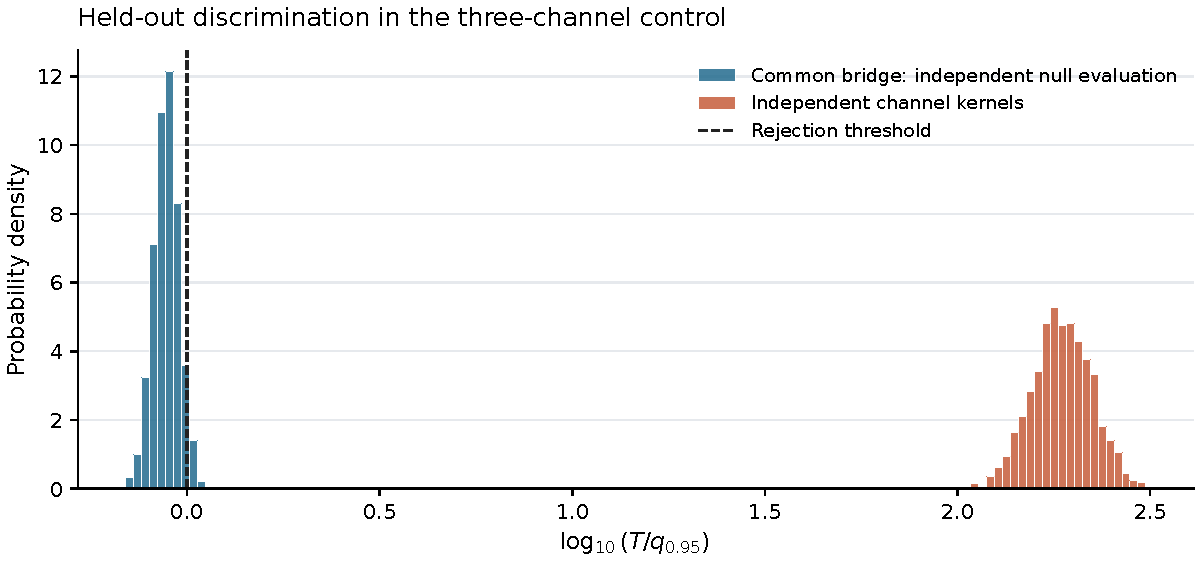
\includegraphics[width=0.75\textwidth]{bridge_synthetic_residuals.pdf}
\caption{Held-out synthetic discrimination. The horizontal variable is the base-ten logarithm of the statistic normalized by the preregistered 95-percent common-bridge threshold. The common-bridge distribution has the declared five-percent rejection rate; the independent-kernel distribution lies far beyond the decision boundary. The figure demonstrates this finite protocol only; it is not evidence for a physical ECL bridge.}
\label{fig:synthetic_bridge}
\end{figure}

The same script records all seeds, dimensions, noise levels, thresholds, and summary statistics in a machine-readable JSON file. It can therefore be rerun without reconstructing hidden choices.

\subsection{Near-saturated counterexample}

Consider two channels with \(p_{\chi}=q_{\chi}=10\), and choose
\begin{equation}
N_{\mathrm{in}}=N_{\mathrm{out}}=r=14.
\end{equation}
Then
\begin{equation}
D_{\mathrm{ind}}=2\times10\times10=200,
\qquad
D_r^{\mathrm{nom}}=14(28-14)=196.
\end{equation}

Because \cref{eq:compression_ratio} is defined through \(D_{\mathrm{tot}}^{\mathrm{eff}}\) and not through \(D_r^{\mathrm{nom}}\), the counterexample must be evaluated on the identifiable image, not on the nominal variety. That is the whole point of \cref{eq:effective_bridge_dimension}, and a negative control that quoted \(D_r^{\mathrm{nom}}\) would silently abandon it. Here the two counts coincide, and the reason is worth stating because it does not always hold.

Since \(r=N_{\mathrm{in}}=N_{\mathrm{out}}=14\), the rank constraint is vacuous and \(\mathcal V_{r}=\mathrm{Hom}(\mathcal H_{\mathrm{br}}^{\mathrm{in}},\mathcal H_{\mathrm{br}}^{\mathrm{out}})\), a linear space of dimension \(196\). The portfolio operator \(\mathcal L_{\mathbf P}\) is then a linear map \(\mathbb R^{196}\to\mathbb R^{200}\), and
\begin{equation}
\ker\mathcal L_{\mathbf P}
=\left\{
K:\;
K\!\left(\operatorname{Ran}P_{\chi}^{\mathrm{in}}\right)
\subseteq\ker P_{\chi}^{\mathrm{out}}
\ \text{ for }\chi=1,2
\right\}.
\label{eq:counterexample_kernel}
\end{equation}
For generic maps with \(\dim\operatorname{Ran}P_{\chi}^{\mathrm{in}}=10\) inside a \(14\)-dimensional space and \(\dim\ker P_{\chi}^{\mathrm{out}}=4\), the two channels impose \(200\) independent linear conditions on \(196\) unknowns, so \(\ker\mathcal L_{\mathbf P}=\{0\}\) generically and
\begin{equation}
D_{\mathrm{br}}^{\mathrm{eff}}=196,
\qquad
D_{\mathrm{gauge}}=0
\ \text{(frozen maps, \cref{rem:gauge_counting})},
\qquad
\rho_{\mathrm{cap}}=\frac{196}{200}=0.98.
\end{equation}
The construction is therefore genuinely near-saturated in the identifiable sense and not merely in the nominal one. Its rejection is real.

A merely strict inequality \(D_{\mathrm{tot}}^{\mathrm{eff}}<D_{\mathrm{ind}}\) would accept it. Any materially compressive ceiling rejects it, and the specific value \(\rho_{\max}=0.25\) used in \cref{sec:synthetic} is far from the binding consideration: every \(\rho_{\max}<0.98\) rejects this construction, which is the substantive content of the example. The demonstration is that a quantitative margin must be part of the hypothesis, not that \(0.25\) is the correct margin.

\section{Selector naturality and what the bridge forbids}
\label{sec:naturality}

Let \(\chi\to\chi'\) be an arrow only when two selectors have been independently identified as physically equivalent presentations of one corridor. With declared comparison maps \(U_{\chi'\chi}\) and \(V_{\chi'\chi}\), naturality requires
\begin{equation}
K_{\chi'}
=V_{\chi'\chi}K_{\chi}U_{\chi'\chi}^{-1}
\label{eq:naturality}
\end{equation}
within preregistered uncertainty. Orientation-preserving relabeling of one foliation supplies the canonical case. Different materials, carriers, phases, or boundaries are not automatically equivalent; they are constrained by the common anchored bridge, not by exact conjugacy.

The amended bridge forbids:
\begin{enumerate}[leftmargin=1.55em]
\item automatic direct sums or one latent block per channel;
\item near-saturated latent models exceeding \(\rho_{\max}\);
\item invisible bridge directions counted as empirical compression;
\item channel maps jointly estimated from the anomaly data;
\item one independent coordinate gauge per channel;
\item bridge metrics selected to manufacture pseudoinverse agreement;
\item tolerances inflated after residuals are observed;
\item zero-overlap channels described as mutually confirming;
\item physically equivalent selectors producing incompatible kernels;
\item evidence transferred between QI's laboratory and galactic branches without a covariant acceleration bridge.
\end{enumerate}

\section{QI branch separation and the inertial portfolio}
\label{sec:qi_branches}

The independent audit shows that the Unruh relation uses proper acceleration while QI's galactic applications use acceleration relative to surrounding matter. The two branches are therefore
\begin{equation}
\mathrm{QI}_{\mathrm{lab}}
=\mathrm{QI}[a_{\mathrm{prop}},\Bdy,\text{carrier}],
\qquad
\mathrm{QI}_{\mathrm{gal}}
=\mathrm{QI}[a_{\mathrm{rel}},U^{\mu},\Theta,\text{orbit}],
\end{equation}
with no derived covariant identification between \(a_{\mathrm{prop}}\) and \(a_{\mathrm{rel}}\). A capacitor confirmation would support only the laboratory branch; a galactic fit would support only the galactic branch. The two branches may enter one common-bridge portfolio only after the preparation maps encode a single independently specified covariant acceleration object or action.

This is not merely a caution about interpretation. If the laboratory and galactic responses require irreducibly different input objects, no fixed channel maps into one anchored bridge coordinate system can make them two readouts of one inertial law without adding a new bridge. Their apparent corroboration would then be a category error.

A second axis of separation must be declared alongside the first, and it is sharper than a closure ambiguity. The audit reconstructs the primary galactic derivation and finds that the QI floor relation and the Tully--Fisher relation are specializations of one closure applied to a decomposed acceleration \(|A|=|a|+|a'|\), where \(a\) is the mean orbital acceleration and \(a'\) an unresolved ensemble of small-scale motions, and where the summation domain of \(|A|\) is never specified \cite{ArellanoQIAudit2026}.

This matters directly for the portfolio, because an unspecified summation domain is fatal to channel-map anchoring in a way that a mere closure ambiguity would not be. Route~A and route~B both require \(P_{\chi}^{\mathrm{in}}\) to be fixed before the target anomalies are inspected, and \(P_{\chi}^{\mathrm{in}}\) acts on a declared finite input space \(\mathcal A_{\chi}\). If the physical input variable is a sum of acceleration magnitudes over a matter set that the analyst chooses, then \(\mathcal A_{\chi}\) is not fixed by the channel's physics and the map can be tuned after the fact through the choice of summation aperture. That is precisely the joint re-estimation forbidden by item~4 of \cref{sec:naturality}, arriving through the input space rather than through the map.

The portfolio declaration must therefore state, for every entry, the acceleration object, the closure, and---where a relational acceleration is used---the explicit summation domain that makes the channel input computable from the system's description alone. A portfolio that fails to do so is not admissible under \cref{prot:bridge}, irrespective of how well the bridge subsequently fits.

\section{Failure jurisdiction and evidentiary symmetry}
\label{sec:failure}

The final failure rules are symmetric:
\begin{align}
\text{QI branch prediction fails}
&\Longrightarrow
\text{that tested QI branch fails},\\
\text{QI branch succeeds}
&\Longrightarrow
\text{that branch gains support},\\
\rho_{\mathrm{cap}}>\rho_{\max}
\text{ or }\eta_{\mathrm{fit}}>\eta_{\max}
&\Longrightarrow
\text{the proposed bridge protocol fails},\\
\text{held-out residual or naturality test fails}
&\Longrightarrow
\text{the proposed inertial bridge fails},\\
\text{bridge succeeds}
&\Longrightarrow
\text{the finite bridge gains support only},\\
&\phantom{\Longrightarrow}
\text{while A1--A4 remain independently assessed}.
\end{align}
The governing source architecture remains answerable to its own premises, deductions, consistency, and genuine countermodels. The downstream inertial bridge remains answerable to the finite, preregistered empirical tests constructed here. Neither direction is permitted to borrow evidentiary status from the other.

\section{Invariants, artifacts, assumptions, and interpretations}

\begin{longtable}{>{\raggedright\arraybackslash}p{0.23\textwidth}>{\raggedright\arraybackslash}p{0.20\textwidth}>{\raggedright\arraybackslash}p{0.49\textwidth}}
\toprule
Object or claim & Status & Required treatment \\
\midrule
A1--A4 and typed ECL architecture & Governing framework premise & Not inferred from the synthetic bridge or from QI. \\
Finite bridge-coordinate spaces & Conditional representation & Never identified with Counterspace or the complete ECL. \\
\(\mathbb K_{\mathrm{br}}\) & Frozen finite bridge operator & Rank, metric, coordinate convention, and training data fixed before target comparison. \\
\(D_{\mathrm{br}}^{\mathrm{eff}}\) & Identifiable model dimension & Computed from the image of the rank variety under the fixed portfolio operator. \\
\(P_{\chi}^{\mathrm{in/out}}\) & Source-derived or calibration-derived maps & Count their parameters unless independently fixed; prohibit per-channel gauges. \\
Low-rank compression & Testable bridge hypothesis & Requires \(\rho_{\mathrm{cap}}\le\rho_{\max}\) computed on the identifiable image, data sufficiency, and held-out predictive success. \\
Linearized channel kernels & Scope restriction & \(K_{\chi}^{\mathrm{obs}}\) is a Fr\'echet derivative at a declared base point; the protocol tests linearized responses only, never the full nonlinear maps. \\
\(\Sigma_{\chi}^{\mathrm{bridge}}\) & Mandatory covariance term & Propagated uncertainty of the fitted bridge; omitting it makes the residual test anti-conservative. \\
\(D_{\mathrm{gauge}}\) & Accounting convention & Applies to estimated maps only; zero for frozen maps, since \(D_{\mathrm{br}}^{\mathrm{eff}}\) is already gauge-invariant. \\
QI closure reading & Resolved source-side & Both published astrophysical relations use one implicit closure; the open issue is the undeclared summation domain of \(|A|=|a|+|a'|\), which leaves the channel input space unfixed and so blocks admissible map anchoring. \\
Moore--Penrose reconstruction & Metric-dependent mathematical tool & Interpreted only on channel-readable bridge sectors. \\
Positivity or stability & Standard admissibility requirement & Not evidence for ECL. \\
Synthetic acceptance--rejection result & Executed protocol demonstration & Establishes exclusion power of the finite test, not physical truth of the bridge. \\
QI laboratory/galactic unification & Open bridge & Requires one covariant acceleration definition and common action or response law. \\
\bottomrule
\end{longtable}

\section{Discussion}

\subsection{What has become non-vacuous}

Low rank alone does not establish a source relation. The amended content is the conjunction of: an identifiable image dimension; a material compression margin; independent coordinate anchoring; one residual global gauge; metric-fixed pseudoinverses; parameter-to-data sufficiency; covariance-based tolerances; a powered held-out test against independent kernels; and a nontrivial shared readable sector. Removing any one of these conditions reopens a route to accommodation.

\subsection{Relationship to system identification}

Shared latent-state and subspace-identification methods already demonstrate how several input--output records can be represented through a lower-dimensional state model \cite{Ljung1999,VanOverscheeDeMoor1996}. The present paper does not claim that low-rank or multi-view identification is unique to TCGS. Its conditional framework contribution is the source--Shadow jurisdiction assigned to a successfully identified shared bridge and the prohibition against treating that bridge as source-exhaustive. The mathematical test must still stand on ordinary identifiability, calibration, and predictive grounds.

\subsection{What the synthetic example proves and does not prove}

The worked example proves that the proposed finite protocol has a nonempty accepted class and a demonstrable rejected class under declared settings. It closes the objection that the alleged forbidden region exists only verbally. It does not show that real inertial channels share a rank-two bridge, that route-B calibration can be executed across galaxies and capacitors, or that the bridge is generated by ECL. Those remain empirical and constructive tasks.

\subsection{Constructive frontier}
\label{sec:frontier}

The highest-value next step is a real multi-channel calibration study in a regime where standardized perturbations, independent channel maps, and overlapping readable sectors can be measured. A laboratory portfolio involving distinct mechanical and electromagnetic carriers is more appropriate than combining a capacitor and a galaxy immediately. Only after a common covariant acceleration and channel maps have been fixed should the astrophysical branch enter the same bridge test.

A concrete candidate portfolio makes the requirement checkable rather than aspirational. Three carriers with genuinely different constitutive physics but a common controllable perturbation are: a torsion pendulum read interferometrically; a cryogenic optomechanical resonator; and a cold-atom interferometer. The shared standardized perturbation is a calibrated, reversible, low-frequency inertial drive of declared amplitude applied identically to all three, with the drive waveform, amplitude, and frequency band frozen in advance. Overlap of the readable sectors is then engineered rather than hoped for, by matching the drive bandwidth to a common window in all three response spaces.

Under \cref{sec:linearization} each carrier supplies its base point \(u_{\chi}^{0}\), amplitude \(\epsilon_{\chi}\), and measured linearity residual \(\Lambda_{\chi}\); route~B of \cref{sec:anchoring} supplies one shared coordinate system estimated from the drive campaign alone; and a fourth carrier held back entirely provides the held-out channel required by \cref{prot:bridge}. This portfolio is within reach of a single well-equipped laboratory, which is the point. A protocol that can only be executed by combining a capacitor bench with a galaxy survey is not yet a protocol.

\section{Conclusion}

\begin{tcolorbox}[title=Final classification,colback=white,colframe=black]
This paper supplies a conditional, strongly compressed, independently anchored, globally gauge-fixed, non-exhaustive, and executable common-bridge protocol. It does not derive inertia from A1--A4 and does not establish Quantized Inertia as an expression of ECL.
\end{tcolorbox}

An unrestricted factorization through a latent operator is vacuous. A merely strict parameter inequality is also inadequate: a model retaining 98 percent of unrestricted capacity can satisfy it. The amended bridge is restrictive only because its visible image dimension is computed on the identifiable quotient, its total fitted capacity lies below a preregistered compression ceiling and calibration-data ceiling, its bridge coordinates and metrics are anchored independently, its channel maps share one global gauge rather than per-channel gauges, and its held-out residuals are evaluated at a declared noise floor and power.

Non-exhaustive readability is implemented rather than asserted. Moore--Penrose pseudoinverses reconstruct only partial bridge operators on channel-readable sectors; agreement is required only on a nontrivial shared sector with propagated covariance, and \cref{lem:absorption} shows that this agreement holds under exact factorization precisely when the projectors are orthogonal with respect to the anchored metric, which is why the metric may not be chosen after the residuals are seen. The finite bridge spaces are not named as the source. They are one empirically accessible representation of a proposed common source-conditioned response.

The scope is correspondingly narrow and is stated rather than left implicit: the test concerns linearized channel responses about one declared source configuration, not the full nonlinear maps, and its capacity accounting is performed on the identifiable image rather than the nominal rank variety. The included synthetic example demonstrates actual acceptance and rejection under a fixed design. The QI case then supplies a stringent physical boundary: laboratory proper acceleration and galactic relational acceleration are not interchangeable. Until one covariant bridge is derived, those branches cannot corroborate each other and should not be forced into one inertial portfolio.

The resulting evidentiary discipline is symmetric. Failure rejects the bridge proposed here. Success supports that bridge only. Counterspace and the ECL are neither protected by every downstream failure nor confirmed by every downstream success. That separation is the framework-preserving route by which a source--Shadow inertial programme can acquire genuine empirical content.

\appendix

\section{Rank-variety and effective-image dimensions}

For a real \(N_{\mathrm{out}}\times N_{\mathrm{in}}\) matrix of exact rank \(r\), write \(K=UV\), where \(U\in\mathbb R^{N_{\mathrm{out}}\times r}\) and \(V\in\mathbb R^{r\times N_{\mathrm{in}}}\). The transformation
\begin{equation}
(U,V)\mapsto(UG,G^{-1}V),
\qquad G\in\mathrm{GL}(r),
\label{eq:rank_factor_gauge}
\end{equation}
leaves \(K\) unchanged. The generic rank-manifold dimension is therefore \(D_r^{\mathrm{nom}}=r(N_{\mathrm{in}}+N_{\mathrm{out}}-r)\). With fixed channel maps, the empirical model dimension is the rank of the differential of \(\mathcal L_{\mathbf P}\) on the tangent space, as in \cref{eq:local_effective_dimension}. If the maps annihilate a tangent direction, that direction is not identifiable and cannot be counted as supported compression.

\section{Coordinate gauge, metrics, and pseudoinverse jurisdiction}

The global gauge in \cref{eq:global_gauge} preserves all channel kernels. Once bridge metrics are fixed by calibration, arbitrary general-linear transformations no longer preserve the Moore--Penrose inverse. Whitening and axis anchoring reduce the admissible gauge to metric-preserving transformations; sign and ordering conventions remove nondegenerate residual ambiguities. If the calibration leaves an exactly degenerate subspace, only gauge-invariant quantities on that block may enter the test.

For finite matrix \(P\), the Moore--Penrose inverse satisfies
\begin{equation}
PP^{+}P=P,
\quad
P^{+}PP^{+}=P^{+},
\quad
(PP^{+})^{*}=PP^{+},
\quad
(P^{+}P)^{*}=P^{+}P.
\end{equation}
Thus \(PP^{+}\) and \(P^{+}P\) are orthogonal projectors only relative to the declared metrics. Pseudoinverse agreement therefore cannot be claimed before the bridge inner products and coordinate convention are fixed.

\section{Synthetic algorithm and reproducibility}

The included script \texttt{code/bridge\_synthetic\_demo.py} performs the following steps:
\begin{enumerate}[leftmargin=1.55em]
\item generate and freeze three channel-map pairs using an independent seed;
\item generate common-bridge or independent-kernel calibration and held-out data;
\item fit one shared bridge operator on calibration data only;
\item enforce the rank bound by truncated singular-value decomposition;
\item calibrate the held-out threshold from a separate common-bridge Monte Carlo sample;
\item estimate empirical size and power on independent replicate sets;
\item export the figure and a JSON file containing all fixed settings and results.
\end{enumerate}
The demonstration ceiling \(\rho_{\max}=0.25\) belongs to this synthetic design only and is not proposed as a universal physical constant.

\section{Preregistration checklist}

\begin{longtable}{>{\raggedright\arraybackslash}p{0.27\textwidth}>{\raggedright\arraybackslash}p{0.65\textwidth}}
\toprule
Item & Required declaration \\
\midrule
Channel portfolio & Physical systems, operating regimes, equivalent-selector arrows, and inequivalent carriers. \\
Empirical spaces & Discretization, preprocessing, dimensions, metrics, and retained observables for every \(\mathcal A_{\chi}\) and \(\mathcal F_{\chi}\). \\
Linearization & Base point \(u_{\chi}^{0}\), perturbation amplitude \(\epsilon_{\chi}\), probe design, kernel estimator, linearity tolerance \(\tau_{\chi}\), and the declared physical closure for every channel. \\
Anchoring route & Source-derived or independent calibration-derived; calibration interventions and data split. \\
Bridge coordinates & \(N_{\mathrm{in}}\), \(N_{\mathrm{out}}\), inner products, whitening, axis order, sign convention, and residual global gauge. \\
Rank and image capacity & \(r\), \(D_r^{\mathrm{nom}}\), \(D_{\mathrm{br}}^{\mathrm{eff}}\), invisible directions, and computation method. \\
Total fitted capacity & Map, nuisance, and bridge parameter counts, with \(D_{\mathrm{gauge}}\) reported together with the rank computation that produced it (\cref{rem:gauge_counting}). \\
Compression and data ceilings & \(\rho_{\max}\), \(\eta_{\max}\), and their design justification. \\
Predictive covariance & Measurement, calibration, map, discretization, and serial-dependence components. \\
Held-out power & \(\alpha_*\), \(1-\beta_*\), \(\Delta_{\min}\), effective sample size, and multiplicity rule. \\
Comparison model & Independent per-channel kernels \cref{eq:independent_null} and the held-out predictive score \(\mathcal S\) used in \cref{eq:predictive_comparison}. \\
Simulation alternative & The independent-kernel data-generating process used for the power calculation, reported separately from the comparison model. \\
Shared sector & Algorithm for identifying nontrivial common readable sectors and handling non-comparability. \\
Revision rule & Any change in portfolio, coordinates, rank, maps, tolerance model, or threshold defines a new model version. \\
QI branch rule & Laboratory and galactic branches remain separate until one covariant acceleration bridge is frozen; every portfolio entry declares both its acceleration object and its closure. \\
\bottomrule
\end{longtable}

\section{Notation dictionary}
\label{app:notation}

\begin{tabularx}{\textwidth}{>{\raggedright\arraybackslash}p{0.25\textwidth}X}
\toprule
Symbol & Meaning \\
\midrule
\(\Cfour\) & Complete non-temporal Counterspace source domain. \\
\(\Shadow\) & Operationally real three-dimensional Shadow. \\
\(\Xi,\Xi_0\) & Complete admissible source configuration and reference configuration. \\
\(\ECL_{\Sset,\Xi}\) & Complete selector-indexed ECL readability profile. \\
\(\chi\) & Complete physical channel, including selector, carrier, corridor, and boundary data. \\
\(\mathcal A_{\chi},\mathcal F_{\chi}\) & Finite empirical input and output spaces of channel \(\chi\). \\
\(\mathcal H_{\mathrm{br}}^{\mathrm{in/out}}\) & Finite shared bridge-coordinate spaces; not the complete source. \\
\(N_{\mathrm{in}},N_{\mathrm{out}}\) & \emph{Dimensions} of \(\mathcal H_{\mathrm{br}}^{\mathrm{in}}\) and \(\mathcal H_{\mathrm{br}}^{\mathrm{out}}\). Roman letters; scalars. \\
\(\Kout\) & \emph{Portfolio-blind subspace} \(\bigcap_{\chi}\ker P_{\chi}^{\mathrm{out}}\subseteq\mathcal H_{\mathrm{br}}^{\mathrm{out}}\). Script letter; a subspace, not a dimension. Distinct from \(N_{\mathrm{out}}\). \\
\(\mathcal H_{\mathrm{in}}^{\mathrm{id}},\mathcal H_{\mathrm{out}}^{\mathrm{id}}\) & Identifiable input span and output quotient \(\mathcal H_{\mathrm{br}}^{\mathrm{out}}/\Kout\). \\
\(\mathbb K_{\mathrm{br}}\) & Frozen rank-bounded common bridge operator. \\
\(P_{\chi}^{\mathrm{in/out}}\) & Source-derived or independently calibration-derived channel maps. \\
\(\mathcal L_{\mathbf P}\) & Portfolio operator mapping one bridge operator to the family of channel kernels. \\
\(\mathfrak M_{r,\mathbf P}\) & Visible rank-bounded common-bridge model family. \\
\(D_{\mathrm{br}}^{\mathrm{eff}}\) & Dimension of the identifiable visible image. \\
\(D_{\mathrm{tot}}^{\mathrm{eff}}\) & Total fitted capacity after map, nuisance, and gauge accounting. \\
\(\rho_{\mathrm{cap}},\eta_{\mathrm{fit}}\) & Compression ratio and parameter-to-calibration-data ratio. \\
\(\Pi_{\chi}^{\mathrm{in/out}}\) & Projectors onto bridge directions readable through channel \(\chi\). \\
\(T_{\chi},T_{\chi\chi'}\) & Channel and shared-sector Mahalanobis statistics. \\
\(\Sigma_{\chi}^{\mathrm{bridge}}\) & Propagated uncertainty of the fitted bridge operator in \cref{eq:predictive_covariance}. \\
\(u_{\chi}^{0},\epsilon_{\chi},\tau_{\chi},\Lambda_{\chi}\) & Linearization base point, perturbation amplitude, declared linearity tolerance, and measured second-order residual. \\
\(\mathcal S\) & Held-out predictive score used in the model comparison \cref{eq:predictive_comparison}. \\
\(D_{\mathrm{gauge}}\) & Gauge-orbit dimension on the joint map-and-bridge parameter; zero for frozen maps. \\
\(a_{\mathrm{prop}},a_{\mathrm{rel}}\) & Proper and as-yet undefined covariant relational accelerations. \\
\(\mathrm{QI}_{\mathrm{lab}},\mathrm{QI}_{\mathrm{gal}}\) & Laboratory and galactic QI branches before covariant unification. \\
\bottomrule
\end{tabularx}

\section*{Declarations}

\paragraph{Author contributions.}
Conceptualization, formal analysis, methodology, investigation, software supervision, and writing: H.A.-P. The author assumes responsibility for the final manuscript.

\paragraph{Funding.}
No external funding was received.

\paragraph{Competing interests.}
The author develops TCGS--SEQUENTION and declares no other competing interest.

\paragraph{Data and code availability.}
No new experimental dataset was generated. The source package includes the complete LaTeX and BibTeX files, the fixed synthetic-demonstration script, the machine-readable result file, and the generated figure. The synthetic data are generated deterministically from the seeds declared in the script.

\paragraph{Use of computational tools.}
Computational tools supported source organization, algebraic checks, simulation, figure generation, bibliography preparation, and LaTeX compilation. The author assumes responsibility for all claims and interpretations.

\paragraph{License.}
This manuscript is distributed under the Creative Commons Attribution 4.0 International License, except for externally cited works, which retain their own licenses.

\bibliographystyle{unsrtnat}
\bibliography{TCGS_QI_TCGS_BRIDGE_COMPANION_REFERENCES_FINAL_V4_AUG2026}

\end{document}
